% =====================================================================
% Draft section — sparse Walsh recovery via compressed sensing.
%
% Argument: the pairwise Walsh interaction spectrum can be recovered
% from O(k) random coalitions rather than 2^n exhaustive ones,
% because the interaction spectrum of real circuits is effectively
% sparse. This makes Walsh-based interaction analysis practical for
% circuits with 20+ heads.
%
% Status: v1 first draft. Compiles standalone.
% Requires: booktabs, amsmath, graphicx, natbib (\citet/\citep).
% =====================================================================

\subsection{Sparse recovery scales coalition sweeps beyond 15 heads}
\label{sec:sparse-walsh-recovery}

A coalition sweep over $n$ heads requires $2^n$ forward passes: 32\,768
for 15~heads, feasible but slow; ${\sim}10^6$ for 20~heads, borderline;
${\sim}10^9$ for 30, impossible. The exponential cost confines Walsh
interaction analysis to small circuits.  Compressed
sensing~\citep{candes2005decoding} offers an alternative: sample $M \ll 2^n$
random coalitions, build the corresponding rows of the Walsh basis matrix
$\Phi_{mc} = (-1)^{\mathrm{popcount}(c \,\&\, s)}$, and solve a sparse
regression for the $k = n + \binom{n}{2}$ order-1 and order-2 coefficients.
If the interaction spectrum is compressible, recovery succeeds at $M$
far below $2^n$.

\paragraph{Theoretical brackets.}

Two sample-complexity regimes bound the required $M$. The generic RIP
bound for Gaussian or Bernoulli measurement matrices gives
$M = O(k \log(N/k))$~\citep{candes2005decoding}; for $k=210$ and
$N = 2^{20}$, this is $M \approx 1400$. Our measurement matrix is a
subsampled Walsh--Hadamard matrix, where the tighter structured bound
$M = O(k \log k \log N)$ applies~\citep{bourgain2014,rudelson2008sparse},
with a matching lower bound $\Omega(k \log k \log(N/k))$ from
\citet{blasiok2019sparse}. For the same parameters this gives $M \approx 13\,000$.
Recovery should become reliable somewhere between these bounds.

\paragraph{Methods.}

Three recovery algorithms were compared. LASSO with cross-validated
regularization (LassoCV, 5-fold) selects both which coefficients are nonzero
and their magnitudes. Orthogonal matching pursuit with cross-validated
sparsity (OrthogonalMatchingPursuitCV, 5-fold) makes the same selection
greedily. Neither method receives oracle knowledge of $k$. Monte Carlo
direct estimation, $\hat{w}_S = M^{-1} \sum_c f(c)\, \chi_S(c)$, serves as
an unbiased but high-variance baseline.

\paragraph{Phase~1: validation on existing exact sweeps.}

Fourteen completed exact sweeps (15-head IOI and RTI circuits under three
ablation primitives, $k = 120$, $N = 32\,768$) provided ground truth. At
each sample size $M$, ten random subsets of the full $2^n$ coalition values
were drawn, and sparse recovery was compared to the exact Walsh spectrum.
LASSO achieved $r > 0.95$ at $M = 100$ ($M/k = 0.83$) and $r > 0.99$ at
$M = 500$ ($M/k = 4.2$) across all fourteen circuits, with OMP trailing by
a small margin. Monte Carlo required $M > 2000$ for $r > 0.85$.

\paragraph{Phase~2: a 20-head circuit where exact sweeps are infeasible.}

The top 20 attention heads for IOI in GPT-2 small were identified by
activation patching (mean ablation of each of 144~heads on 200~IOI prompts,
ranked by change in logit difference). The resulting circuit has
$k = 20 + \binom{20}{2} = 210$ target coefficients and $2^{20} \approx 10^6$
possible coalitions. Two thousand random coalitions were evaluated (each
requiring one forward pass with a random subset of the 20~heads mean-ablated),
and pairwise Walsh coefficients were recovered via LASSO and OMP.

\medskip

\begin{tabular}{rrccccc}
\toprule
$M$ & $M/k$ & Compression & LASSO $r$ & OMP $r$ & MC $r$ & Top-10 recall \\
\midrule
  100 & 0.48 &  10\,486$\times$ & $0.91 \pm 0.02$ & $0.85 \pm 0.04$ & $0.24 \pm 0.07$ & 83\% \\
  140 & 0.67 &   7\,490$\times$ & $0.96 \pm 0.01$ & $0.94 \pm 0.02$ & --- & 91\% \\
  200 & 0.95 &   5\,243$\times$ & $0.98 \pm 0.00$ & $0.98 \pm 0.01$ & $0.33 \pm 0.04$ & 93\% \\
  500 & 2.38 &   2\,097$\times$ & $1.00 \pm 0.00$ & $1.00 \pm 0.00$ & $0.50 \pm 0.04$ & 97\% \\
 2000 & 9.52 &     524$\times$ & $1.00 \pm 0.00$ & $1.00 \pm 0.00$ & $0.77 \pm 0.00$ & 100\% \\
\bottomrule
\end{tabular}

\medskip

Recovery reaches $r > 0.95$ at $M = 140$ ($M/k = 0.67$), meaning fewer
random coalitions are needed than there are coefficients to recover. The
effective sparsity of the interaction spectrum is far below the nominal
$k = 210$: LASSO selects roughly 50--80 nonzero coefficients at the
threshold $M$, and the remaining coefficients are small enough that
regularization correctly zeros them. Split-half validation --- two
independent LASSO recoveries from disjoint 1000-coalition subsets ---
yields $r = 0.997$ between the two estimates.

Figure~\ref{fig:sparse-walsh-recovery}(a) traces the full recovery curve from
$M = 20$ to $M = 2000$. LASSO dominates OMP at small $M$ and the two converge
above $M/k \approx 1$. Monte Carlo remains below $r = 0.8$ even at
$M = 2000$, confirming that sparse regression is essential --- random
sampling alone does not exploit the compressibility.
Figure~\ref{fig:sparse-walsh-recovery}(b) overlays the 20-head and 15-head
recovery curves as a function of $M/k$. The curves collapse: recovery
quality depends on samples per coefficient, not on circuit size.

\begin{figure}[t]
\centering
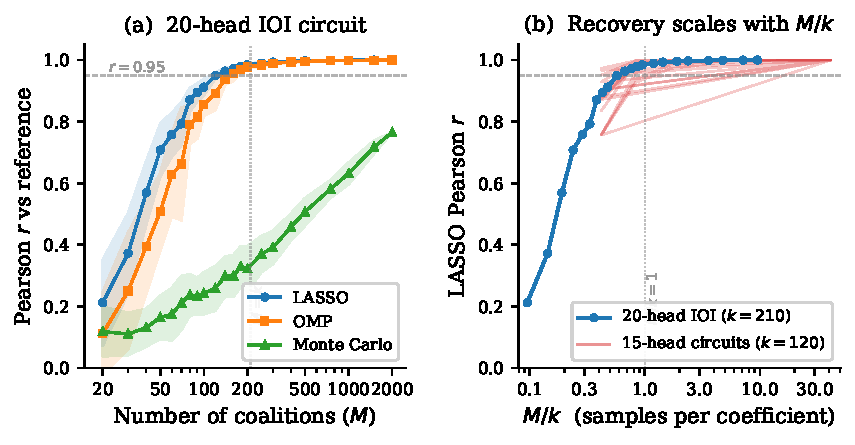
\includegraphics[width=\textwidth]{figures/sparse_walsh_recovery.pdf}
\caption{Sparse Walsh recovery of pairwise interaction coefficients.
\textbf{(a)}~Recovery quality (Pearson~$r$ vs.\ $M{=}2000$ reference) for the
20-head IOI circuit in GPT-2 small. LASSO crosses $r = 0.95$ at $M = 140$
($7\,490\times$ compression over exact enumeration). Shaded bands show
$\pm 1$ s.d.\ across 20 random trials.
\textbf{(b)}~LASSO recovery across circuits of different sizes, plotted
against $M/k$ (samples per target coefficient). Fourteen 15-head circuits
from Phase~1 (light lines) and the 20-head circuit (dark line) follow the
same curve, confirming that the sample complexity scales with the number of
coefficients, not with the number of coalitions.}
\label{fig:sparse-walsh-recovery}
\end{figure}

\paragraph{Walsh interaction vs.\ EAP edge attribution.}

The recovered Walsh coefficients measure actual coalition interaction: how
much the joint ablation of heads $i$ and $j$ deviates from the sum of their
individual effects. EAP edge scores~\citep{syed2023attribution} measure
linearized gradient flow between heads. Comparing the magnitude-ranked
pairwise Walsh coefficients to the corresponding EAP edge products gives
Spearman $\rho = 0.58$ and Pearson $r = 0.73$. The two methods agree on
which pairs interact most strongly --- the top interacting pair by both
measures is L8H6--L5H5, two name movers --- but diverge on weaker pairs
where nonlinear routing effects dominate. The moderate correlation supports
the thesis that different discovery methods impose different selective
pressures on the interaction structure they recover: Walsh coefficients
capture the full nonlinear interaction, while EAP captures the linear
component.

\paragraph{Scaling implications.}

For a circuit of 30~heads ($k = 465$, $N \approx 10^9$), recovery at
$M/k = 1$ requires roughly 500 forward passes --- a ten-minute GPU job
rather than an impossible enumeration. At 50~heads ($k = 1275$), the
cost is ${\sim}1300$ forward passes. Sparse Walsh recovery transforms
the interaction analysis from a small-circuit diagnostic into a scalable
circuit discovery method, applicable wherever activation patching can
identify a candidate head set.
